\begin{center}
    \textbf{Teoría Clásica del Consumidor. Fundamentos.}
\end{center}

\begin{center}
\textbf{Prof. Javier Hervés Estévez}
\end{center}

\begin{center}
\textbf{Alumno: Christian Limbert Paredes Aguilera}
\end{center}

\begin{center}
	\rule{0.5\textwidth}{0.4pt}
\end{center}
\vspace{.8cm}

\begin{enumerate}[\textbf{Ejercicio} \bfseries 1.]

    %-------------------- 1.
    \item \textbf{Comprobar que el conjunto presupuestario de un agente no cambia si los precios se triplican.}\\

	\textbf{Solución:} Sea $\overline{\omega}^i = \left(\overline{\omega}_1^i,\ldots,\overline{\omega}_L^i\right)\in \mathbb{R}^L_+$ donde $\overline{\omega}^i_l$ es la dotación del bien $l$ adquirida por el consumidor $i$. Definamos la renta y el gasto como:
	$$M^i\left(\overline{\textbf{p}}\right)=\left[\overline{\textbf{p}}\, \overline{\omega}^i=\displaystyle\sum_{l=1}^L \overline{\textbf{p}}_l \,\overline{\omega}_l^i\right]; \qquad \overline{\textbf{p}}\textbf{x}^i=\displaystyle\sum_{l=1}^L \overline{\textbf{p}}_l x_l^i$$
	respectivamente. Dado que el conjunto presupuestario está definido como:
	$$\beta^i\left(\overline{\textbf{p}}\right)=\hat{\beta}^i\left[\overline{\textbf{p}},M^i\left(\overline{\textbf{p}}\right)\right]=\left\{\textbf{x}^i\in \mathcal{X}^i:\overline{\textbf{p}}\textbf{x}^i\leq M^i\left(\overline{\textbf{p}}\right)\left[=\overline{\textbf{p}} \,\overline{\omega}^i\right]\right\}.$$
	Podemos suponer que los precios se triplican, es decir, $\overline{\textbf{p}}\rightarrow 3\overline{\textbf{p}}$. Por lo tanto, el conjunto presupuestario viene dado por:
	$$\beta^i\left(3\overline{\textbf{p}}\right)=\left\{\textbf{x}^i\in \mathcal{X}^i:3\overline{\textbf{p}}\textbf{x}^i\leq M^i\left(3\overline{\textbf{p}}\right)\right\}$$
	De donde,
	$$
	\begin{array}{rcl}
	    3\overline{\textbf{p}}\,\overline{\textbf{x}}^i & \leq & M^i\left(3\overline{\textbf{p}}\right)\\\\
	    \displaystyle\sum_{l=1}^L \left(3\overline{\textbf{p}}_l\right) \,\overline{\textbf{x}}_l^i & \leq & \displaystyle\sum_{l=1}^L \left(3\overline{\textbf{p}}_l\right) \,\overline{\omega}_l^i\\\\
	    3\overline{\textbf{p}}_1 \,\overline{\textbf{x}}_1^i + \ldots + 3\overline{\textbf{p}}_L \,\overline{\textbf{x}}_L^i & \leq & 3\overline{\textbf{p}}_1 \,\overline{\omega}_1^i + \ldots + 3\overline{\textbf{p}}_L \,\overline{\omega}_L^i\\\\
	    3\left(\overline{\textbf{p}}_1 \,\overline{\textbf{x}}_1^i + \ldots + \overline{\textbf{p}}_L \,\overline{\textbf{x}}_L^i\right) & \leq & 3\left(\overline{\textbf{p}}_1 \,\overline{\omega}_1^i + \ldots + \overline{\textbf{p}}_L \,\overline{\omega}_L^i\right)\\\\
	    \overline{\textbf{p}}_1 \,\overline{\textbf{x}}_1^i + \ldots + \overline{\textbf{p}}_L \,\overline{\textbf{x}}_L^i & \leq & \overline{\textbf{p}}_1 \,\overline{\omega}_1^i + \ldots + \overline{\textbf{p}}_L \,\overline{\omega}_L^i\\\\
	    \displaystyle\sum_{l=1}^L \overline{\textbf{p}}_l \,\overline{\textbf{x}}_l^i & \leq & \displaystyle\sum_{l=1}^L \overline{\textbf{p}}_l \,\overline{\omega}_l^i\\\\
	    \overline{\textbf{p}}\,\overline{\textbf{x}}^i & \leq & M^i\left(\overline{\textbf{p}}\right).
	\end{array}
	$$

	Por lo tanto,
	$$\beta^i\left(\overline{\textbf{p}}\right)=\left\{\textbf{x}^i\in \mathcal{X}^i:\overline{\textbf{p}}\textbf{x}^i\leq M^i\left(\overline{\textbf{p}}\right)\right\}$$
	Así, el conjunto presupuestario no cambia si los precios se triplican.\\\\


    %-------------------- 2.
    \item \textbf{Demostrar que si los precios de los bienes son positivos. Entonces, el conjunto presupuestario es compacto y convexo (en nuestro contexto, un conjunto es compacto si es a la vez cerrado y acotado).}\\

	\textbf{Solución:} Para demostrar que el conjunto presupuestario es convexo si los precios de los bienes son positivos, necesitamos mostrar que para cualquier par de cestas de bienes $\textbf{x}^i$ e $\textbf{y}^i$ en el conjunto presupuestario, la cesta 
	$$\alpha\textbf{x}^i + (1-\alpha)\textbf{y}^i$$ 
	también está en el conjunto presupuestario para cualquier $\alpha \in [0,1]$. Dado que $\textbf{x}^i$ e $\textbf{y}^i$ están en el conjunto presupuestario y $\overline{p}$ positivo, tenemos que:
	$$\overline{\textbf{p}}\textbf{x}^i\leq M^i\left(\overline{\textbf{p}}\right) \qquad \land \qquad \overline{\textbf{p}}\textbf{y}^i\leq M^i\left(\overline{\textbf{p}}\right)$$
	De donde, podemos multiplicar por $\alpha$ y $(1-\alpha)$ respectivamente
	$$\alpha\overline{\textbf{p}}\textbf{x}^i\leq \alpha M^i\left(\overline{\textbf{p}}\right) \qquad \land \qquad (1-\alpha)\overline{\textbf{p}}\textbf{y}^i\leq (1-\alpha)M^i\left(\overline{\textbf{p}}\right)$$
	Luego, sumamos las dos desigualdades:
	$$\alpha\overline{\textbf{p}}\textbf{x}^i + (1-\alpha)\overline{\textbf{p}}\textbf{y}^i\leq \alpha M^i\left(\overline{\textbf{p}}\right) + (1-\alpha)M^i\left(\overline{\textbf{p}}\right)$$
	Por definición de gasto,
	$$\sum_{l=1}^L \alpha\overline{\textbf{p}}_l\textbf{x}_l^i + \sum_{l=1}^L (1-\alpha)\overline{\textbf{p}}_l\textbf{y}_l^i\leq M^i(\textbf{p}).$$
	Por propiedades de sumatorias,
	$$
	\begin{array}{rcl}
	    \displaystyle\sum_{l=1}^L \overline{\textbf{p}}_l\left[\alpha\textbf{x}_l^i + (1-\alpha)\textbf{y}_l^i\right] &\leq& M^i(\textbf{p})\\\\
	    \overline{\textbf{p}}\left[\alpha\textbf{x}^i + (1-\alpha)\textbf{y}^i\right] &\leq& M^i(\textbf{p})
	\end{array}
	$$
	Hemos dicho que los bienes $\textbf{x}^i$ e $\textbf{y}^i$ están en el conjunto presupuestario y $\alpha \in [0,1]$. Por lo que se cumple la definición de \textbf{convexidad}. Así,
	$$\beta^i\left(\overline{\textbf{p}}\right)=\left\{\textbf{x}^i, \textbf{y}^i\in \mathcal{X}^i:\overline{\textbf{p}}\left[\alpha\textbf{x}^i + (1-\alpha)\textbf{y}^i\right]\leq M^i(\textbf{p})\right\}.$$

	Para demostrar que el conjunto presupuestario es compacto, necesitamos mostrar que el conjunto presupuestario es cerrado y acotado. Primero demostremos que es cerrado. Un conjunto es cerrado si contiene todos sus puntos límite y un punto límite de un conjunto es un punto tal que cualquier entorno del punto contiene al menos un punto del conjunto.\\

	En el caso del conjunto presupuestario, consideremos una secuencia de cestas de bienes $\{\textbf{x}^i_k\}$ en el conjunto presupuestario que converge a una cesta límite $\textbf{x}^i$. Esto significa que para cualquier $\epsilon > 0$, existe un $K$ tal que para todo $k > K$, tenemos que la distancia 
	$$\|\textbf{x}^i_k - \textbf{x}^i\| < \epsilon.
	\footnote{
	Esta notación $\epsilon$-$K$ es una forma estándar de definir la convergencia de una secuencia en análisis matemático. Significa que, más allá de cierto punto en la secuencia (es decir, para todo $k > K$), los términos de la secuencia están arbitrariamente cerca del límite $\textbf{x}^i$. Dado que cada $\textbf{x}^i_k$ está en el conjunto presupuestario, tenemos que $\overline{\textbf{p}}\textbf{x}^i_k\leq M^i\left(\overline{\textbf{p}}\right)$ para todo $k$. 
	}
	$$
	Dado que cada $\textbf{x}^i_k$ está en el conjunto presupuestario, tenemos que 
	$$\overline{\textbf{p}}\textbf{x}^i_k\leq M^i\left(\overline{\textbf{p}}\right)$$ 
	para todo $k$. Ahora, dado que $\textbf{x}^i_k$ converge a $\textbf{x}^i$, tenemos que 
	$$\overline{\textbf{p}}\textbf{x}^i_k \text{ converge a } \overline{\textbf{p}}\textbf{x}^i.$$ 
	Es decir, $\displaystyle\lim_{k \to \infty} \overline{\textbf{p}}\textbf{x}^i_k = \overline{\textbf{p}}\textbf{x}^i$.
	Por lo tanto, tenemos que 
	$$\lim_{k \to \infty} \overline{\textbf{p}}\textbf{x}^i_k = \overline{\textbf{p}}\textbf{x}^i \leq m^i\left(\overline{\textbf{p}}\right).$$
	Esto demuestra que $\textbf{x}^i$ está en el conjunto presupuestario, lo que demuestra que el conjunto presupuestario
	$$\beta^i\left(\overline{\textbf{p}}\right)=\left\{\textbf{x}^i\in \mathcal{X}^i:\lim_{k \to \infty} \overline{\textbf{p}}\textbf{x}^i_k=\overline{\textbf{p}}\textbf{x}^i\leq M^i\left(\overline{\textbf{p}}\right)\right\}$$
	es \textbf{cerrado}.\\

	Ahora, para demostrar que el conjunto presupuestario es acotado. Es suficiente demostrar que todos los elementos del conjunto; en este caso la cesta de bienes $x_k^i$ son menores o iguales a un número finito. Para ello podemos tomar la desigualdad de Cauchy-Schwarz, donde
	$$
	\begin{array}{rcl}
	    \overline{\textbf{p}}\textbf{x}^i_k &\leq& \|\overline{\textbf{p}}\|\|\textbf{x}^i_k\|\\\\
	    M(\overline{\textbf{p}}) &\leq& \|\overline{\textbf{p}}\|\|\omega^i_k\|\\\\
	\end{array}
	$$
	Sumando las desigualdades, tenemos que
	$$\overline{\textbf{p}}\textbf{x}^i_k + M(\overline{\textbf{p}}) \leq \|\overline{\textbf{p}}\|\|\textbf{x}^i_k\| + \|\overline{\textbf{p}}\|\|\omega^i_k\|.$$
	Dado que $\overline{\textbf{p}}$ es positivo, despejamos $\textbf{x}^i_k$ de la siguiente manera:
	$$\|\textbf{x}^i_k\| \leq \dfrac{\overline{\textbf{p}}\textbf{x}^i_k + M(\overline{\textbf{p}})}{\|\overline{\textbf{p}}\|} + \|\omega^i_k\|.$$
	En vista de que $\frac{\overline{\textbf{p}}\textbf{x}^i_k + M(\overline{\textbf{p}})}{\|\overline{\textbf{p}}\|} + \|\omega^i_k\|$ es un número finito. Entonces, concluimos que el conjunto presupuestario es \textbf{acotado}. De esta manera hemos demostrado que el conjunto presupuestario es \textbf{convexo}, \textbf{cerrado} y \textbf{acotado}, por lo tanto, es \textbf{compacto}.\\\\

    %-------------------- 3.
    \item \textbf{\boldmath Un consumidor posee unas preferencias lexicográficas sobre $x=(x_1,x_2)\in \mathbb{R}^2_+$ si la relación de preferencias verifica que $x\succ y$ si $x_1>y_1$ o, en el caso que $x_1=y_1$ entonces $x\succ y$ si $x_2>y_2$. Conteste a las siguientes preguntas:}

	\begin{enumerate}[\bfseries a)]

	    %---------- a.
	    \item \textbf{Dibuje un mapa de indiferencia para estas preferencias.}\\
		\begin{center}
		    \begin{tikzpicture}
			\draw[->] (0,0) -- (5,0) node[right] {$x_1$};
			\draw[->] (0,0) -- (0,5) node[above] {$x_2$};

			\foreach \x in {1,2,3,4} {
			    \draw (\x,0) -- (\x,5-\x) node[above right] {$I_\x$};
			}
		    \end{tikzpicture}
		\end{center}


	    %---------- b.
	    \item \textbf{Verificar que la ordenación lexicográfica es completa, transitiva, monótona y estrictamente convexa.}\\

		\textbf{Solución:}

		\begin{itemize}

		    \item \textbf{Completitud:} Para cualquier par de bienes $x, y \in \mathbb{R}^2_+$, se cumple que $x \succ y$, $y \succ x$ o $x \sim y$. Esto se debe a que, por definición, comparamos primero la primera componente y luego la segunda. Por lo tanto, siempre podemos establecer una relación de preferencia entre cualquier par de bienes.

		    \item \textbf{Transitividad:} Si $x \succ y$ e $y \succ z$, entonces $x \succ z$. Esto se sigue directamente de la definición de las preferencias lexicográficas. Si $x_1 > y_1$ e $y_1 > z_1$, entonces $x_1 > z_1$. Si $x_1 = y_1$ e $y_1 = z_1$, pero $x_2 > y_2$ e $y_2 > z_2$, entonces $x_2 > z_2$.

		    \item \textbf{Monotonía:} Si $x_1 > y_1$ o si $x_1 = y_1$ pero $x_2 > y_2$, entonces $x \succ y$. Esto significa que si tenemos más de al menos uno de los bienes, entonces preferimos ese paquete de bienes, lo cual es consistente con la definición de las preferencias lexicográficas.

		    \item \textbf{Estrictamente convexa:} Aquí es donde las preferencias lexicográficas difieren de muchas otras preferencias. Las preferencias lexicográficas no son estrictamente convexas. La estricta convexidad implica que preferimos la diversificación. Sin embargo, en las preferencias lexicográficas, si $x \succ y$, entonces siempre preferiremos tener más del bien 1, incluso si eso significa tener menos del bien 2. Por lo tanto, no preferimos necesariamente una cesta diversificada de bienes.\\

		\end{itemize}

	    %---------- c.
	    \item \textbf{\boldmath Piense en qué falla el siguiente argumento: “Las preferencias lexicográficas no son convexas porque dadas dos cestas, existen cestas intermedias que son más preferidas; por ejemplo, dadas las cestas $x = (2, 2)$ e $y = (4, 0)$, la cesta $z = (3, 1)$, correspondiente a $\lambda = 0.5$, verifica que $z\succ_i x$, pues $z_1>x_1$, pero $y \succ z$, pues $y_1 > z_1$.”}.\\

		\textbf{Solución:} Las preferencias lexicográficas se definen de tal manera que un bien se considera superior a otro si su primera coordenada es mayor, o si la primera coordenada es igual pero la segunda coordenada es mayor. Esto significa que la primera coordenada tiene prioridad absoluta en la decisión. \\

		En particular se tiene dos cestas, $x = (2, 2)$ e $y = (4, 0)$, y una cesta intermedia $z = (3, 1)$, que es una combinación convexa de $x$ e $y$ con $\lambda = 0.5$.\\

		Según las preferencias lexicográficas, $z$ es preferido a $x$ porque $z_1 > x_1$, sin importar los valores de $z_2$ y $x_2$. Del mismo modo, $y$ es preferido a $z$ porque $y_1 > z_1$, sin importar los valores de $y_2$ y $z_2$.\\

		Esto es consistente con las preferencias lexicográficas, pero contradice la noción de convexidad. La convexidad en el sentido de las preferencias implica que cualquier combinación convexa de dos cestas es al menos tan preferida como las cestas originales. Pero en este caso, aunque $z$ es una combinación convexa de $x$ e $y$, no es cierto que $z$ sea al menos tan preferido como $x$ e $y$.\\

		Por lo tanto, las preferencias lexicográficas no son convexas. \\

	    %---------- d.
	    \item \textbf{¿Por qué no se pueden representar las preferencias lexicográficas por una función de utilidad?; ¿qué características tienen los conjuntos indiferentes? (¿cómo son los conjuntos indiferentes?); ¿qué axioma de las preferencias no cumple este criterio de ordenación?}.\\

		\textbf{Solución:} Primeramente, las preferencias lexicográficas no pueden ser representadas por una función de utilidad continua. Esto se debe a que las preferencias lexicográficas dan prioridad absoluta a un bien sobre otro, lo que significa que no hay compensación entre bienes. En otras palabras, no importa cuánto aumente la cantidad del segundo bien, nunca compensará una disminución en la cantidad del primer bien. Esto contradice la suposición de continuidad que se requiere para la representación de utilidad.\\

		Los conjuntos indiferentes son líneas rectas paralelas al eje de uno de los bienes. Esto se debe a que, para un nivel dado del primer bien, el consumidor es indiferente a la cantidad del segundo bien. Por lo tanto, todos los paquetes de bienes que tienen la misma cantidad del primer bien pero diferentes cantidades del segundo bien se encuentran en el mismo conjunto indiferente.\\

		Por último, la ordenación lexicográfica no cumple con el axioma de la convexidad. La convexidad implica que, entre dos cestas preferidas, cualquier combinación convexa de ellas también es preferida. Sin embargo, en las preferencias lexicográficas, esto no es cierto. Como mencioné antes, no importa cuánto aumente la cantidad del segundo bien, nunca compensará una disminución en la cantidad del primer bien.\\

	\end{enumerate}

    %-------------------- 4.
    \item \textbf{Considere las siguientes funciones de utilidad (Villar 1999, Ejercicio 3.9):}

	\begin{enumerate}[\bfseries a)]

	    %---------- a.
	    \item \textbf{Dibuje un mapa de indiferencia para cada una de estas utilidades.}\\

	    \begin{enumerate}[i)]

		\item \textbf{\boldmath (utilidades lineales) $u(x_1,x_2)=\alpha_1x_1+\alpha_2x_2$.}\\

		\begin{multicols}{3}
		    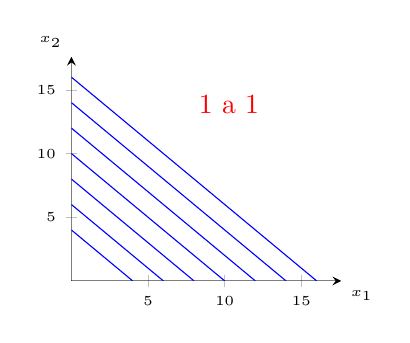
\begin{tikzpicture}
			\begin{axis}[scale=.5,draw opacity =.5,samples=100,smooth, 
			  axis x line=center, 
			  axis y line=center,
			  ylabel = {$x_2$},
			  xlabel = {$x_1$},
			  xlabel style={below right},
			  ylabel style={above left},
			  label style={font=\tiny},
			  tick label style={font=\tiny},
			  enlargelimits=upper] 
			  \foreach \i in {4,6,...,16} {
			    \addplot[blue,opacity=1,domain=0:\i]{(\i-\x)/1};
			   }
			\end{axis}
			  \draw[red](2,2)node[above]{$1$ a $1$};
		    \end{tikzpicture}
		    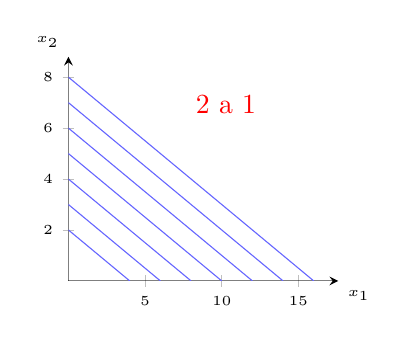
\begin{tikzpicture}
			\begin{axis}[scale=.5,draw opacity =.5,samples=100,smooth, 
			  axis x line=center, 
			  axis y line=center,
			  ylabel = {$x_2$},
			  xlabel = {$x_1$},
			  xlabel style={below right},
			  ylabel style={above left},
			  label style={font=\tiny},
			  tick label style={font=\tiny},
			  enlargelimits=upper] 
			  \foreach \i in {4,6,...,16} {
			    \addplot[blue!60,opacity=1,domain=0:\i]{(\i-\x)/2};
			   }
			\end{axis}
			  \draw[red](2,2)node[above]{$2$ a $1$};
		    \end{tikzpicture}
		    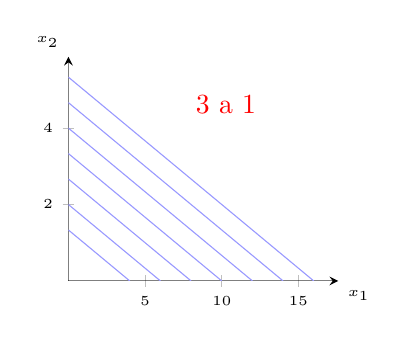
\begin{tikzpicture}
			\begin{axis}[scale=.5,draw opacity =.5,samples=100,smooth, 
			  axis x line=center, 
			  axis y line=center,
			  ylabel = {$x_2$},
			  xlabel = {$x_1$},
			  xlabel style={below right},
			  ylabel style={above left},
			  label style={font=\tiny},
			  tick label style={font=\tiny},
			  enlargelimits=upper] 
			  \foreach \i in {4,6,...,16} {
			    \addplot[blue!40,opacity=1,domain=0:\i]{(\i-\x)/3};
			   }
			\end{axis}
			  \draw[red](2,2)node[above]{$3$ a $1$};
		    \end{tikzpicture}
		\end{multicols}

		\item \textbf{\boldmath (utilidades tipo Leontief) $u(x_1,x_2)=\min\{x_1, x_2\}$.}\\
		    \begin{center}
			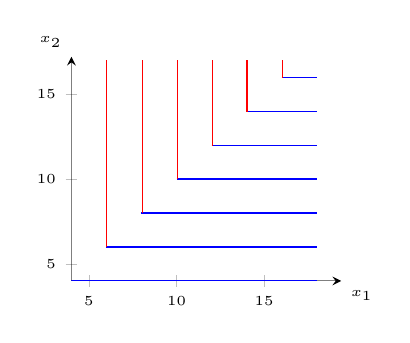
\begin{tikzpicture}
			    \begin{axis}[scale=.5,draw opacity =.5,samples=100,smooth, 
			      axis x line=center, 
			      axis y line=center,
			      ylabel = {$x_2$},
			      xlabel = {$x_1$},
			      xlabel style={below right},
			      ylabel style={above left},
			      label style={font=\tiny},
			      tick label style={font=\tiny},
			      enlargelimits=upper] 
			      \foreach \i in {4,6,...,16} {
				\addplot[blue,opacity=1,domain=\i:18]{\i};
			       }
			    \end{axis}
			       \draw[red](.45,.43)--(.45,2.8);
			       \draw[red](.9,.86)--(.9,2.8);
			       \draw[red](1.35,1.29)--(1.35,2.8);
			       \draw[red](1.79,1.72)--(1.79,2.8);
			       \draw[red](2.23,2.15)--(2.23,2.8);
			       \draw[red](2.68,2.58)--(2.68,2.8);
			\end{tikzpicture}
		    \end{center}

		\item \textbf{\boldmath (utilidades tipo Cobb-Douglas) $u(x_1,x_2)=x_1^{\alpha}x_2^{1-\alpha}$}\\
		    \begin{center}
			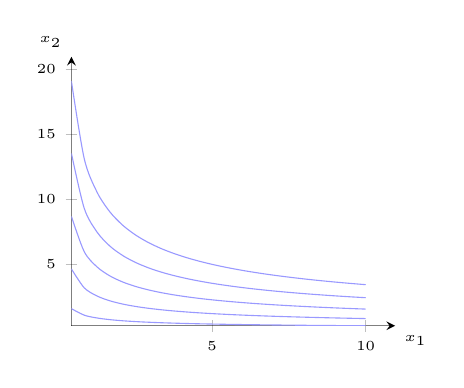
\begin{tikzpicture}
			    \begin{axis}[scale=.6,draw opacity =.5,smooth, 
			      axis x line=center, 
			      axis y line=center,
			      ylabel = {$x_2$},
			      xlabel = {$x_1$},
			      xlabel style={below right},
			      ylabel style={above left},
			      label style={font=\tiny},
			      tick label style={font=\tiny},
			      enlargelimits=upper] 
			      \foreach \i in {1,...,5} {
				\addplot[blue!40,opacity=1,domain=0:10]{((\i/\x^(1-0.65))^(1/0.65)};
			       }
			    \end{axis}
			\end{tikzpicture}
		    \end{center}

		\item \textbf{\boldmath (utilidades CES) $u(x_1,x_2)=\left[\alpha_1 x_1^{\rho}+\alpha_2 x_2^{\rho}\right]^{1/\rho}$}\\
		    \begin{center}
			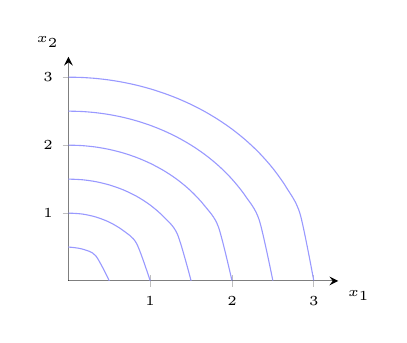
\begin{tikzpicture}
			    \begin{axis}[scale=.5,draw opacity =.5,smooth, 
			      axis x line=center, 
			      axis y line=center,
			      ylabel = {$x_2$},
			      xlabel = {$x_1$},
			      xlabel style={below right},
			      ylabel style={above left},
			      label style={font=\tiny},
			      tick label style={font=\tiny},
			      enlargelimits=upper] 
			      \foreach \i in {.5,1,...,3} {
				\addplot[blue!40,opacity=1,domain=0:4]{( (\i^2-1*\x^2)/1 )^(1/2)};
			       }
			    \end{axis}
			\end{tikzpicture}
		    \end{center}
	    \end{enumerate}
	    \vspace{.5cm}

	    % ---------- b)
	    \item \textbf{Compruebe que todas son funciones de utilidad homogéneas y de qué grado.}\\

	    \begin{enumerate}[i)]

		\item \textbf{\boldmath (utilidades lineales) $u(x_1,x_2)=\alpha_1x_1+\alpha_2x_2$.}\\

		    Recordemos que una función $f(x_1, x_2)$ es homogénea de grado $k$ si, al multiplicar todos sus argumentos por un número $t > 0$, la función se multiplica por $t^k$. Es decir, debe cumplir con la siguiente propiedad:
		    $$f(tx_1, tx_2) = t^kf(x_1, x_2)$$
		    Ahora, consideremos la función de utilidad lineal 
		    $$u(x_1,x_2)=\alpha_1x_1+\alpha_2x_2.$$ 
		    Queremos ver si esta función es homogénea y de qué grado. Si multiplicamos ambos argumentos de la función por $t$, obtenemos:
		    $$u(tx_1, tx_2) = \alpha_1(tx_1) + \alpha_2(tx_2)$$
		    Simplificando, obtenemos:
		    $$u(tx_1, tx_2) = t(\alpha_1x_1 + \alpha_2x_2)$$

		    Observa que $t(\alpha_1x_1 + \alpha_2x_2)$ es exactamente $t$ veces la función original $u(x_1, x_2)$. Por lo tanto, la función se multiplica por $t$ cuando todos sus argumentos se multiplican por $t$. Esto es exactamente la definición de una función homogénea de grado 1.\\

		    Así, concluimos que la función de utilidad lineal $u(x_1,x_2)=\alpha_1x_1+\alpha_2x_2$ es homogénea de grado 1.\\\\


		\item \textbf{\boldmath (utilidades tipo Leontief) $u(x_1,x_2)=\min\{x_1, x_2\}$.}\\

		    Para verificar si la función de utilidad de Leontief $u(x_1,x_2)=\min\{x_1, x_2\}$ es homogénea y de qué grado, necesitamos ver cómo se comporta cuando todos sus argumentos se multiplican por un número $t > 0$.\\ 
s
		    Dado que sabemos que 
		    $$\min\{x_1, x_2\}=\dfrac{x_1+x_2-|x_2-x_1|}{2},$$ 
		    podemos reescribir la función de utilidad como 
		    $$u(x_1,x_2)=\dfrac{x_1+x_2-|x_2-x_1|}{2}.$$
		    Si multiplicamos ambos argumentos de la función por $t$, obtenemos:
		    $$u(tx_1, tx_2) = \dfrac{tx_1+tx_2-|tx_2-tx_1|}{2} = t\dfrac{x_1+x_2-|x_2-x_1|}{2} = tu(x_1, x_2)$$
		    Por lo tanto, la función se multiplica por $t$ cuando todos sus argumentos se multiplican por $t$. Esto es exactamente la definición de una función homogénea de grado 1.\\

		    Así, podemos concluir que la función de utilidad de Leontief $u(x_1,x_2)=\min\{x_1, x_2\}$ es homogénea de grado 1. \\\\

		\item \textbf{\boldmath (utilidades tipo Cobb-Douglas) $u(x_1,x_2)=x_1^{\alpha}x_2^{1-\alpha}$}\\

		    Para verificar si esta función es homogénea y de qué grado, necesitamos ver cómo se comporta cuando todos sus argumentos se multiplican por un número $t > 0$. Si multiplicamos ambos argumentos de la función por $t$, obtenemos:
		    $$u(tx_1, tx_2) = (tx_1)^{\alpha}(tx_2)^{1-\alpha} = t^{\alpha}x_1^{\alpha}t^{1-\alpha}x_2^{1-\alpha} = t^{\alpha + 1 - \alpha}(x_1^{\alpha}x_2^{1-\alpha}) = tu(x_1, x_2).$$

		    Por lo tanto, la función se multiplica por $t$ cuando todos sus argumentos se multiplican por $t$. Esto es exactamente la definición de una función homogénea de grado 1.\\

		    Así, podemos concluir que la función de utilidad Cobb-Douglas $u(x_1,x_2)=x_1^{\alpha}x_2^{1-\alpha}$ es homogénea de grado 1. \\\\

		\item \textbf{\boldmath (utilidades CES) $u(x_1,x_2)=\left[\alpha_1 x_1^{\rho}+\alpha_2 x_2^{\rho}\right]^{1/\rho}$}\\

		    Para comprobar si la función de utilidad $u(x_1,x_2)=\left[\alpha_1 x_1^{\rho}+\alpha_2 x_2^{\rho}\right]^{1/\rho}$ es homogénea, sustituimos $x_1$ y $x_2$ por $tx_1$ y $tx_2$ respectivamente:
		    $$u(tx_1,tx_2)=\left[\alpha_1 (tx_1)^{\rho}+\alpha_2 (tx_2)^{\rho}\right]^{1/\rho}.$$
		    Simplificamos la ecuación:
		    $$u(tx_1,tx_2)=\left[t^{\rho}\alpha_1 x_1^{\rho}+t^{\rho}\alpha_2 x_2^{\rho}\right]^{1/\rho}.$$
		    Factorizamos $t^{\rho}$:
		    $$u(tx_1,tx_2)=\left[t^{\rho}(\alpha_1 x_1^{\rho}+\alpha_2 x_2^{\rho})\right]^{1/\rho}.$$
		    Finalmente, obtenemos:
		    $$u(tx_1,tx_2)=t(\alpha_1 x_1^{\rho}+\alpha_2 x_2^{\rho})^{1/\rho}=tu(x_1,x_2).$$
		    Por lo tanto, la función de utilidad es homogénea de grado 1.\\\\

	    \end{enumerate}

	    %---------- c)
	    \item \textbf{\boldmath Compruebe que las preferencias representadas por las funciones i), ii) y iii) son las mismas que las preferencias representadas a partir de la iv) (es decir, que las curvas de indiferencia y, por tanto, la relación marginal de sustitución para las funciones i), ii) y iii) son las mismas que las que se obtienen para iv)) en los siguientes casos: i) $\rho = 1$, ii) $\rho \to -\infty$, iii) $\rho\to 0$.}\\

	    La relación marginal de sustitución (MRS) viene dado por:
	    $$MRS_{x_1,x_2}=-\dfrac{\partial u/\partial x_1}{\partial u/\partial x_2}.$$
	    Ahora, el MRS de la función CES se calcula cómo sigue:
	    $$\dfrac{\partial F}{\partial x_i} = \alpha_ix_i^{\theta-1}\left(\alpha_1x_1^{\theta}+\alpha_2x_2^{\theta}\right)^{\frac{1-\theta}{\theta}}.$$
	    Entonces, la MRS es:
	    $$MRS_{x_1,x_2}=-\dfrac{\alpha_1x_1^{\theta-1}\left(\alpha_1x_1^{\theta}+\alpha_2x_2^{\theta}\right)^{\frac{1-\theta}{\theta}}}{\alpha_2x_2^{\theta-1}\left(\alpha_1x_1^{\theta}+\alpha_2x_2^{\theta}\right)^{\frac{1-\theta}{\theta}}}=-\dfrac{\alpha_1x_1^{\theta-1}}{\alpha_2x_2^{\theta-1}}.$$
	    Debido a que el cambio porcentual de una función viene dado por la derivada de su valor logaritmo, la ecuación de arriba implica:
	    $$\text{El cambio de porcentaje de } MRS_{x_1,x_2} \text{ en } \dfrac{x_2}{x_1} = \dfrac{d\ln MRS_{x_1,x_2}}{d(x_2,x_1)} = \dfrac{1-\theta}{x_2/x_1}.$$
	    Definamos $\rho$ como la elasticidad de sustitución entre $x_1$ y $x_2$:
	    $$\rho = \dfrac{\% \text{ cambio de "indice de consumo"}}{\% \text{ cambio de "tasa marginal de sustitución"} (MRS_{x_1,x_2})}\qquad (1)$$
	    Por lo tanto,
	    $$\rho = \dfrac{d\ln(x_2/x_1)}{d\ln MRS_{x_1,x_2}} = \dfrac{1}{1-\theta}.$$
	    Sabemos que $\rho = 0$ si $u$ es Leontief, $\rho = 1$ si $u$ es lineal. Para el caso lineal sólo nos queda sustituir $\theta=-2$. Para Leontief no es sencillo verlo, pero al final vemos que converge.\\

	    De manera similar, la convergencia a la función CobbDouglas no es sencilla. La función Cobb-Douglas está definida por
	    $$u(x_1,x_2)=x_1^{\alpha}x_2^{1-\alpha}.$$
	    donde $\alpha\in (0,1)$ se sabe que es la proporción del consumo de $x_1$ (de modo que $1-\alpha$ es el de $x_2$). Así,
	    $$\dfrac{\partial u}{\partial x_1} = \alpha \left(\dfrac{x_1}{x_2}\right)^{\alpha-1} \qquad \text{y}\qquad \dfrac{\partial u}{\partial x_2} = (1-\alpha) \left(\dfrac{x_2}{x_1}\right)^{\alpha}.$$
	    Entonces, definimos:
	    $$MRS_{x_1,x_2} = \dfrac{\partial u / \partial x_1}{\partial f / \partial x_2} = \dfrac{\alpha}{1-\alpha} \dfrac{x_1}{x_2}.$$
	    Esto implica que,
	    $$\%\text{ cambio de } MRS_{x_1,x_2} \text{ en } \dfrac{x_2}{x_1} = \dfrac{d\ln MRS_{x_1,x_2}}{d(x_2/x_1)} = \dfrac{1}{x_2/x_1}.$$
	    De (1), la participación del consumo es fija y, por lo tanto, $\rho = 1$. Esto significa que la función CES debe converger a Cobb-Douglas como $\theta\to 0$, o $\rho = 1/(1-\theta)\to 1$, aunque no es fácil ver si realmente es así.\\
	    

	    %---------- d)
	    \item \textbf{\boldmath Compruebe: e1) que la función i) se obtiene a partir de la iv) para $\rho = 1$; e2) la función iii) se obtiene a partir de la iv) para $\rho \to 0$ y $\alpha_1 + \alpha_2 = 1$; e3) pero que las funciones ii) y iii), en general, no se obtienen a partir de la iv) para los casos: ii) $\rho \to -\infty$ y iii) $\rho \to 0$.}\\

	    \begin{enumerate}[e1)]

		\item 

		Cuando $\rho = 1$, la función de utilidad CES se convierte en una función de utilidad lineal. Es decir, 
		$$u(x_1,x_2)=\left[\alpha_1 x_1^{1}+\alpha_2 x_2^{1}\right]^{1/1} \quad \Rightarrow \quad u(x_1,x_2)=\alpha_1 x_1+\alpha_2 x_2.$$ 
		Esto es idéntico a la función de utilidad i).\\

		\item 

		Sea la función de utilidad CES:
		$$u(x_1,x_2)=\left[\alpha_1 x_1^{\rho}+\alpha_2 x_2^{\rho}\right]^{1/\rho}.$$
		Donde,
		$$\ln(u)=\dfrac{\ln(\alpha_1 x_1^{\rho}+\alpha_2 x_2^{\rho})}{\rho}.$$
		Aplicamos el límite $\rho \to 0$ y dado que $\alpha_1 + \alpha_2 = 1$:
		$$\lim_{\rho\to 0}\ln(u)=\lim_{\rho\to 0}\dfrac{\ln(\alpha_1 x_1^{\rho}+\alpha_2 x_2^{\rho})}{\rho}=\lim_{\rho\to 0}\dfrac{\ln(\alpha_1 x_1^{0}+\alpha_2 x_2^{0})}{0}=\dfrac{\ln(1)}{0}=\dfrac{0}{0}.$$
		Aplicando la regla de L'Hôpital:
		$$
		\begin{array}{rcl}
		    \displaystyle\lim_{\rho\to 0} \ln(u)&=&\displaystyle\lim_{\rho\to 0} \dfrac{\frac{d}{d\rho}(\ln(\alpha_1 x_1^{\rho}+\alpha_2 x_2^{\rho}))}{\frac{d}{d\rho}\rho}\\\\
					   &=&\displaystyle\lim_{\rho\to 0} \dfrac{\alpha_1 x_1^{\rho}\ln(x_1)+\alpha_2 x_2^{\rho}\ln(x_2)}{\alpha_1 x_1^{\rho}+\alpha_2 x_2^{\rho}}\\\\
					   &=&\dfrac{\alpha_1 \ln(x_1)+\alpha_2 \ln(x_2)}{\alpha_1 +\alpha_2=1}\\\\
					   &=&\alpha_1 \ln(x_1)+\alpha_2 \ln(x_2).
		\end{array}
		$$

		Por lo tanto,
		$$u(x_1,x_2)=x_1^{\alpha}x_2^{1-\alpha}.$$
		Ya que, $\alpha_1 + \alpha_2 = 1$.\\\\


		\item En si la convergencia de la función de utilidad CES a las funciones de utilidad tipo Leontief y Cobb-Douglas en general se da para los casos $\rho\to -\infty$ y $\rho\to 0$, respectivamente. Sea,
		$$\lim_{\rho\to 0,-\infty} \ln (u) = \lim_{\rho\to 0,-\infty} \dfrac{\ln(\alpha_1 x_1^{\rho}+\alpha_2 x_2^{\rho})}{\rho}.$$
		Para cada caso de convergencia, aplicamos la regla de L'Hôpital a $\rho$:
		$$\lim_{\rho\to 0,-\infty} \ln (u) = \lim_{\rho\to 0,-\infty} \dfrac{\alpha_1x_1^\rho\ln(x_1)+\alpha_2x_2^\rho\ln(x_2)}{\alpha_1x_1^\rho+\alpha_2x_2^\rho}.$$
		Para $\rho\to 0$, es sencillo obtener la correspondiente función de Cobb-Douglas:
		$$\lim_{\rho\to 0} \ln (u) = \dfrac{\alpha_1\ln(x_1)+\alpha_2\ln(x_2)}{\alpha_1+\alpha_2} = \alpha_1\ln(x_1)+\alpha_2\ln(x_2).$$
		Cabe mencionar que, si $\alpha_1+\alpha_2=1$ aumenta $u$. Si $\alpha_1+\alpha_2>1$ aumenta $u$ mayor a un factor lineal, y si $\alpha_1+\alpha_2<1$ aumenta $u$ menor a un factor lineal.\\

		Para $\rho\to -\infty$, se obtiene la función de utilidad tipo Leontief, necesitamos algunas manipulaciones técnicas para dividir tanto el numerador como el denominador por $\min\left(x_1,x_2\right)$. De donde,
		$$\displaystyle\lim_{\rho\to -\infty} \dfrac{\alpha_1x_1^\rho\ln(x_1)+\alpha_2x_2^\rho\ln(x_2)}{\alpha_1x_1^\rho+\alpha_2x_2^\rho} = \displaystyle\lim_{\rho\to -\infty} \dfrac{\left[\dfrac{x_1}{\min\left(x_1,x_2\right)}\right]^\rho \ln(x_1)+\left[\dfrac{x_2}{\min\left(x_1,x_2\right)}\right]^\rho \ln(x_2)}{\left[\dfrac{x_1}{\min\left(x_1,x_2\right)}\right]^\rho+\left[\dfrac{x_2}{\min\left(x_1,x_2\right)}\right]^\rho}$$
		$$=\ln\left[\min(x_1,x_2)\right]$$
		Luego, $(x_i/\min(x_1,x_2))^\rho\to 0$ ($\rho\to -\infty$) para $x_i>\min(x_1,x_2)$ y $(x_1/\min(x_1,x_2))^\rho = 1$ para $x_i=\min(x_1,x_2)$ con $x_1\neq x_2$. Posteriormente obtenemos la función de Leontief correspondiente para $\rho\to -\infty$:
		$$\lim_{\rho\to -\infty} (u) =\left[\min(x_1,x_2)\right].$$
		(Esta demostración podemos verificarla en: Saito, Tetsuya, How Do We Get Cobb-Douglas and Leontief Functions from CES Function: A Lecture Note on Discrete and Continuum Differentiated Object Models (May 13, 2011). Journal of Industrial Organization Education, Volume 6, Issue 1 (Article 2), Available at SSRN: \\ https://ssrn.com/abstract=1567152)\\\\

	    \end{enumerate}

	\end{enumerate}

    %-------------------- 5.
    \item \textbf{\boldmath Suponga que las preferencias de un consumidor están representadas por la función de utilidad Cobb-Douglas (continua, monótona y estrictamente cuasicóncava) $u(x_1, x_2) = x_1^\alpha x_2^\beta$ con $\alpha=\beta=1/2$. Se pide:}

	\begin{enumerate}[\bfseries a)]

	    %---------- a)
	    \item \textbf{Mostrar que la función de utilidad es homogénea, e indique de que grado.}\\

		\textbf{Solución:} Empecemos, multiplicando ambos argumentos de la función por $t$:
		$$u(tx_1, tx_2) = (tx_1)^\alpha (tx_2)^\beta$$

		Luego, aplicamos las propiedades de los exponentes para separar $t$:
		$$u(tx_1, tx_2) = t^\alpha x_1^\alpha t^\beta x_2^\beta = t^{\alpha + \beta} x_1^\alpha x_2^\beta$$

		Dado que $\alpha + \beta = 1/2 + 1/2 = 1$, la ecuación se simplifica a:
		$$u(tx_1, tx_2) = t x_1^\alpha x_2^\beta = t u(x_1, x_2)$$

		Por lo tanto, la función de utilidad Cobb-Douglas $u(x_1, x_2) = x_1^\alpha x_2^\beta$ con $\alpha=\beta=1/2$ es homogénea de grado $1$.\\

	    %---------- b)
	    \item \textbf{Las funciones de demanda Marshallianas}.\\

		\textbf{Solución:} Desglosamos el proceso de derivación de las funciones de demanda marshallianas para la función de utilidad Cobb-Douglas $u(x_1, x_2) = x_1^\alpha x_2^\beta$ con $\alpha=\beta=1/2$, sujeta a la restricción presupuestaria $p_1x_1 + p_2x_2 = m$.\\

		Empecemos por maximizar la utilidad del problema del consumidor sujeta a su restricción presupuestaria,
		$$\max_{x_1,x_2} \quad x_1^{1/2} x_2^{1/2}$$
		sujeto a
		$$p_1x_1 + p_2x_2 = m$$

		Para resolver este problema de optimización, podemos formular el Lagrangiano, 
		$$\mathcal{L} = x_1^{1/2} x_2^{1/2} + \lambda(m - p_1x_1 - p_2x_2)$$
		donde $\lambda$ es el multiplicador de Lagrange. Las condiciones de primer orden para un máximo requieren que las derivadas parciales del Lagrangiano con respecto a $x_1$, $x_2$ y $\lambda$ sean iguales a cero:
		$$\frac{\partial \mathcal{L}}{\partial x_1} = \frac{1}{2} x_1^{-1/2} x_2^{1/2} - \lambda p_1 = 0$$
		$$\frac{\partial \mathcal{L}}{\partial x_2} = \frac{1}{2} x_1^{1/2} x_2^{-1/2} - \lambda p_2 = 0$$
		$$\frac{\partial \mathcal{L}}{\partial \lambda} = m - p_1x_1 - p_2x_2 = 0$$

		Si resolvemos las dos primeras ecuaciones para $x_1$ y $x_2$, obtenemos:
		$$x_1 = \left(\frac{x_2^{1/2}}{2\lambda p_1}\right)^2 = \frac{x_2}{4\lambda^2 p_1^2}$$
		$$x_2 = \left(\frac{x_1^{1/2}}{2\lambda p_2}\right)^2 = \frac{x_1}{4\lambda^2 p_2^2}$$

		Sustituyendo $x_1$ en la ecuación de $x_2$, obtenemos:
		$$x_2 = \frac{x_2}{16\lambda^4 p_1^2 p_2^2}$$
		$$16\lambda^4 p_1^2 p_2^2 = 1$$
		$$\lambda^2 = \frac{1}{4\sqrt{p_1 p_2}}$$

		Sustituyendo $\lambda^2$ en las ecuaciones de $x_1$ y $x_2$, obtenemos las funciones de demanda marshallianas correctas:
		$$x_1^* = \frac{m}{2p_1}$$
		$$x_2^* = \frac{m}{2p_2}$$

		Estas funciones de demanda representan la cantidad óptima de cada bien que el consumidor demandará dada su restricción presupuestaria y los precios de los bienes. Como puedes ver, la demanda de cada bien es una función decreciente de su precio y una función creciente del ingreso del consumidor.\\

	    %---------- c)
	    \item \textbf{\boldmath Calcule la cesta óptima para: c1) precios $(p_1,p_2)=(1,4)$ y renta $M=4$, c2) precios $(p_1',p_2)=(4,4)$ y renta $M=4$, c3) precios $(p_1'',p_2=(8,4$ y renta $M=3$. c4) Calcule el nivel de utilidad de la cesta óptima de los apartados c1), c2) y c3). ¿Toma la utilidad un valor positivo o negativo? ¿Qué significa esto?.}\\

		\textbf{Solución:} Vamos a calcular la cesta óptima y el nivel de utilidad para cada caso utilizando las funciones de demanda marshallianas que hemos derivado anteriormente: $x_1^* = \frac{m}{2p_1}$ y $x_2^* = \frac{m}{2p_2}$.

		\begin{enumerate}[\bfseries c1)]

		    \item Para los precios $(p_1,p_2)=(1,4)$ y renta $M=4$, la cesta óptima es:
		    $$x_1^* = \frac{4}{2*1} = 2; \qquad x_2^* = \frac{4}{2*4} = 0.5$$
		    El nivel de utilidad para esta cesta es $u(x_1^*, x_2^*) = (2)^{1/2} * (0.5)^{1/2} = 1$.\\

		    \item  Para los precios $(p_1',p_2')=(4,4)$ y renta $M=4$, la cesta óptima es:
		    $$x_1'^* = \frac{4}{2*4} = 0.5; \qquad x_2'^* = \frac{4}{2*4} = 0.5$$
		    El nivel de utilidad para esta cesta es $u(x_1'^*, x_2'^*) = (0.5)^{1/2} * (0.5)^{1/2} = 0.5$.\\

		    \item  Para los precios $(p_1'',p_2'')=(8,4)$ y renta $M=3$, la cesta óptima es:
		    $$x_1''^* = \frac{3}{2*8} = 0.1875;\qquad x_2''^* = \frac{3}{2*4} = 0.375$$
		    El nivel de utilidad para esta cesta es $u(x_1''^*, x_2''^*) = (0.1875)^{1/2} * (0.375)^{1/2} = 0.2739$.\\

		\end{enumerate}

En todos los casos, la utilidad toma un valor positivo. Esto significa que el consumidor obtiene algún nivel de satisfacción o utilidad de consumir las cestas de bienes. Si la utilidad fuera negativa, significaría que el consumidor está insatisfecho con la cesta de bienes, lo cual no tendría sentido en este contexto ya que el consumidor siempre tiene la opción de no consumir. En la teoría de la utilidad, generalmente asumimos que más consumo es al menos tan bueno como menos consumo, por lo que la utilidad debería ser no negativa.\\

	    %---------- d)
	    \item \textbf{\boldmath Represente gráficamente las curvas de demanda de los bienes 1 y 2 (respecto de sus precios), y sitúe en las curvas de demanda las cestas óptimas obtenidas en c1)-c2)-c3) (Pista.- Recuerde la definición de curva de demanda, y tenga cuidado con los desplazamientos de las curvas).}\\
	    \begin{enumerate}[\bfseries c1)]

		\item \,\\
		    \begin{center}
			    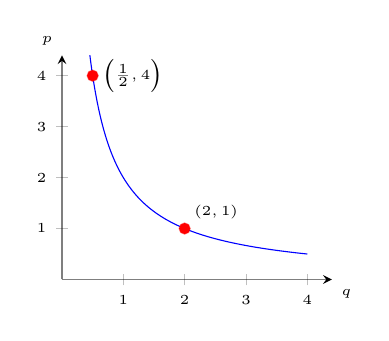
\begin{tikzpicture}
				\begin{axis}[
				  scale=.5,
				  draw opacity =.5,
				  samples=100,
				  smooth, 
				  axis x line=center, 
				  axis y line=center,
				  ylabel = {$p$},
				  xlabel = {$q$},
				  xlabel style={below right},
				  ylabel style={above left},
				  label style={font=\tiny},
				  tick label style={font=\tiny},
				  enlargelimits=upper,
				  xmin=0, xmax=4,  % Aquí se establecen los límites del eje x
				  ymin=0, ymax=4]  % Aquí se establecen los límites del eje y
				\addplot[blue,opacity=1,domain=0:4]{4/(2*\x)};
				\addplot[only marks, mark = *, red] coordinates {(2,1) (.5,4)};
				\node [above right] at (axis cs: 2,1) {\tiny$(2,1)$};
				\node [right] at (axis cs: .5,4) {\tiny$\left(\frac{1}{2},4\right)$};
				\end{axis}
			    \end{tikzpicture}
		    \end{center}
		    \vspace{.5cm}

		\item\;\\ 
		    \begin{center}
			    \begin{tikzpicture}
				\begin{axis}[
				  scale=.5,
				  draw opacity =.5,
				  samples=100,
				  smooth, 
				  axis x line=center, 
				  axis y line=center,
				  ylabel = {$p$},
				  xlabel = {$q$},
				  xlabel style={below right},
				  ylabel style={above left},
				  label style={font=\tiny},
				  tick label style={font=\tiny},
				  enlargelimits=upper,
				  xmin=0, xmax=4,  % Aquí se establecen los límites del eje x
				  ymin=0, ymax=4]  % Aquí se establecen los límites del eje y
				\addplot[blue,opacity=1,domain=0:4]{4/(2*\x)};
				\addplot[only marks, mark = *, red] coordinates {(.5,4) (.5,4)};
				\node [right] at (axis cs: .5,4) {\tiny$\left(\frac{1}{2},4\right)$};
				\end{axis}
			    \end{tikzpicture}
		    \end{center}
		    \vspace{.5cm}

		\item\;\\ 
		    \begin{center}
			    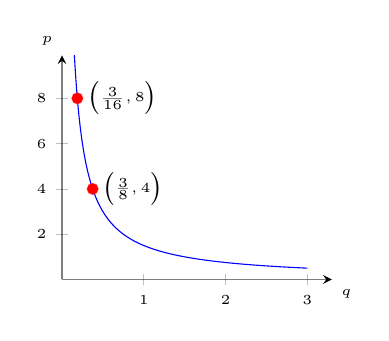
\begin{tikzpicture}
				\begin{axis}[
				  scale=.5,
				  draw opacity =.5,
				  samples=100,
				  smooth, 
				  axis x line=center, 
				  axis y line=center,
				  ylabel = {$p$},
				  xlabel = {$q$},
				  xlabel style={below right},
				  ylabel style={above left},
				  label style={font=\tiny},
				  tick label style={font=\tiny},
				  enlargelimits=upper,
				  xmin=0, xmax=3,  % Aquí se establecen los límites del eje x
				  ymin=0, ymax=9]  % Aquí se establecen los límites del eje y
				\addplot[blue,opacity=1,domain=0:3]{3/(2*\x)};
				\addplot[only marks, mark = *, red] coordinates {(0.1875,8) (0.375,4)};
				\node [right] at (axis cs: 0.1875,8) {\tiny$\left(\frac{3}{16},8\right)$};
				\node [right] at (axis cs: 0.375,4) {\tiny$\left(\frac{3}{8},4\right)$};
				\end{axis}
			    \end{tikzpicture}
		    \end{center}
		    \vspace{.5cm}
	    \end{enumerate}


	    %---------- e)
	    \item \textbf{Calcule la función indirecta de utilidad}\\

		\textbf{Solución:} La función indirecta de utilidad se obtiene sustituyendo las funciones de demanda marshallianas en la función de utilidad. En este caso, nuestras funciones de demanda marshallianas son $x_1^* = \frac{m}{2p_1}$ y $x_2^* = \frac{m}{2p_2}$, y la función de utilidad es $u(x_1, x_2) = x_1^{1/2} x_2^{1/2}$.\\

		Sustituyendo las funciones de demanda en la función de utilidad obtenemos:
		$$v(p_1, p_2, m) = u(x_1^*, x_2^*) = \left(\frac{m}{2p_1}\right)^{1/2} \left(\frac{m}{2p_2}\right)^{1/2} = \frac{m}{2\sqrt{p_1 p_2}}$$

		Esta función nos dice cuál es el nivel máximo de utilidad que puede alcanzar el consumidor dado su ingreso y los precios de los bienes. \\

	    %---------- f)
	    \item \textbf{Obtenga la función de demanda marshalliana a partir de la función indirecta de utilidad.}\\

		\textbf{Solución:} Sea la función indirecta de utilidad  $v(p_1, p_2, m) = \frac{m}{2\sqrt{p_1 p_2}}$. Tomando las derivadas parciales con respecto a $p_1$ y $p_2$, obtenemos:
		$$\frac{\partial v}{\partial p_1} = -\frac{m}{4p_1^{3/2}\sqrt{p_2}}$$
		$$\frac{\partial v}{\partial p_2} = -\frac{m}{4p_2^{3/2}\sqrt{p_1}}$$

		Multiplicando estas derivadas por $-$1, obtenemos las funciones de demanda marshallianas:
		$$x_1^* = \frac{m}{2p_1}$$
		$$x_2^* = \frac{m}{2p_2}$$

		Estas son las mismas funciones de demanda marshallianas que obtuvimos anteriormente a partir de la maximización de la utilidad sujeta a la restricción presupuestaria. Por lo tanto, hemos verificado que nuestras funciones de demanda marshallianas son consistentes con nuestra función indirecta de utilidad. \\\\

	\end{enumerate}
    
    %-------------------- 6.
    \item \textbf{\boldmath Consideremos la siguiente función indirecta de utilidad $v(p,M)=\frac{M}{p_1}+\frac{M}{p_2}$. Calcular:}
	\begin{enumerate}[a)]
	    \item \textbf{La función de demanda normal.}\\

		\textbf{Solución:} La Propiedad de Roy establece que la demanda para el bien $i$ se puede obtener como:
		$$x_i = -\frac{\partial v/\partial p_i}{\partial v/\partial W}$$
		Aplicando la Propiedad de Roy a la función de utilidad indirecta dada, primero calculamos las derivadas parciales necesarias:
		$$
		\left\{
		\begin{array}{rcl}
		    \dfrac{\partial v}{\partial p_1} &=& -\dfrac{M}{p_1^2}\\\\
		    \dfrac{\partial v}{\partial p_2} &=& -\dfrac{M}{p_2^2}\\\\
		    \dfrac{\partial v}{\partial W} &=& \dfrac{1}{p_1} + \dfrac{1}{p_2}.
		\end{array}
		\right.
		$$
		Sustituyendo estas derivadas en la fórmula de la Propiedad de Roy, obtenemos las funciones de demanda Marshallianas para los bienes 1 y 2:
		$$
		\left\{
		    \begin{array}{rcl}
			x_1 = d_1(p,M) &=&-\dfrac{\dfrac{\partial v}{\partial p_1}}{\dfrac{\partial v}{\partial W}} = -\dfrac{-\dfrac{M}{p_1^2}}{\dfrac{1}{p_1} + \dfrac{1}{p_2}} = \dfrac{M}{p_1}.\\\\
			x_2 = d_2(p,M) &=& -\dfrac{\dfrac{\partial v}{\partial p_2}}{\dfrac{\partial v}{\partial W}} = -\frac{-\dfrac{M}{p_2^2}}{\dfrac{1}{p_1} + \dfrac{1}{p_2}} = \dfrac{M}{p_2}.
		    \end{array}
		\right.
		$$

		Estas funciones de demanda indican que la cantidad demandada de cada bien es inversamente proporcional a su precio y directamente proporcional a la renta del consumidor. Es decir, si el precio de un bien aumenta, la cantidad demandada de ese bien disminuye, manteniendo constante la renta del consumidor. Por otro lado, si la renta del consumidor aumenta, la cantidad demandada de cada bien aumenta, manteniendo constantes los precios.\\\\

	    \item \textbf{La función de gasto.}\\

		\textbf{Solución:} La función de gasto a partir de la función de utilidad indirecta, necesitamos despejar $M$ (gasto) en términos de $v$ (nivel de utilidad) y $p$ (precios).\\

		Dada la función de utilidad indirecta $v(p,M)=\frac{M}{p_1}+\frac{M}{p_2}$, podemos reescribirla como:
		$$v = \frac{M}{p_1}+\frac{M}{p_2}.$$
		Multiplicamos ambos lados por $p_1p_2$ para eliminar los denominadores:
		$$v \cdot p_1p_2 = M \cdot p_2 + M \cdot p_1.$$
		Agrupamos los términos de $M$:
		$$M \cdot (p_1 + p_2) = v \cdot p_1p_2.$$
		Finalmente, despejamos $M$ para obtener la función de gasto:
		$$M = \frac{v \cdot p_1p_2}{p_1 + p_2}.$$
		Por lo tanto, la función de gasto es:
		$$e(p,v) = \frac{v \cdot p_1p_2}{p_1 + p_2}.$$\\


	    \item \textbf{La función de demanda compensada.}\\

		\textbf{Solución:} El Lema de Shephard establece que la demanda Hicksiana (o demanda compensada) se obtiene derivando la función de gasto con respecto al precio. En este caso, la función de gasto que obtuvimos anteriormente es:
		$$E(p,v) = \frac{v \cdot p_1p_2}{p_1 + p_2}.$$
		Para obtener la demanda Hicksiana para el bien 1 ($h_1$), derivamos la función de gasto con respecto a $p_1$:
		$$h_1(p,v) = \frac{\partial E(p,v)}{\partial p_1} = \frac{v \cdot p_2(p_1 + p_2) - v \cdot p_1p_2}{(p_1 + p_2)^2} = \frac{v \cdot p_2^2}{(p_1 + p_2)^2}$$
		De manera similar, para obtener la demanda Hicksiana para el bien 2 ($h_2$), derivamos la función de gasto con respecto a $p_2$:
		$$h_2(p,v) = \frac{\partial E(p,v)}{\partial p_2} = \frac{v \cdot p_1^2}{(p_1 + p_2)^2}$$
		Por lo tanto, las funciones de demanda Hicksiana son:
		$$h_1(p,v) = \frac{v \cdot p_2^2}{(p_1 + p_2)^2}$$
		$$h_2(p,v) = \frac{v \cdot p_1^2}{(p_1 + p_2)^2}.$$\\

	\end{enumerate}

    %-------------------- 7.
    \item \textbf{Demostrar el Teorema de Existencia de una función de utilidad continua (ver Jehle).}\\

	\textbf{Solución:} En otras palabras, queremos demostrar que si la relación binaria $\succeq$ es completa, transitiva, continua y estrictamente monótona. Existe, una función real y continua, $u:\mathbb{R}^n_+\to \mathbb{R}$ el cual representa a $\succeq$.\\

	Dado que sólo menciona la existencia podemos afirmar que podría haber por lo menos una función que represente la relación de preferencia. Por lo que si podemos imaginar una sola función que sea continua y que represente las preferencias dadas, habremos demostrado el teorema.\\

	Sea un vector de unos $\textbf{e}\equiv(1,\ldots,1)\in \mathbb{R}^n_+$ y sea $u:\mathbb{R}^n_+\to \mathbb{R}$ tal que,
	\begin{equation}
	    u(\textbf{x})\textbf{e}\sim \textbf{x}.
	\end{equation}
	Es decir, tomamos cualquier $\textbf{x}$ en el dominio de $\mathbb{R}^n_+$ y asignamos el número $u(\textbf{x})$ de manera que el conjunto $u(\textbf{x})e$, con $u(\textbf{x})$ unidades de cada bien sea indiferente a $\textbf{x}$.\\

	Ahora, nos preguntamos ¿si existe siempre un número $u(\textbf{x})$ que satisfaga 1.1? y ¿está determinada de forma única, de modo que $u(x)$ sea una función bien definida?. \\

	Para ver la primera cuestión; sea $\textbf{x}\in \mathbb{R}^n_+$.  Consideremos los dos conjuntos:
	$$
	\begin{array}{rcl}
	    A &\equiv& \left\{t\geq 0: t\textbf{e}\succeq \textbf{x}\right\}\\\\
	    B &\equiv& \left\{t\geq 0: t\textbf{e}\preceq \textbf{x}\right\}
	\end{array}
	$$
	Notemos que si $t^*\in A\cap B$. Entonces, $t^*\textbf{e}\sim \textbf{x}$. Por lo que, $u(\textbf{x})=t^*$ podría satisfacer 1.1. Para ello, demostraremos que $A\cap B$ es no vacío. \\

	Sabemos que la continuidad de $\succeq$ para $A$ y $B$ es cerrada en $\mathbb{R}_+$. También por la Monotonicidad estricta, $t\in A$ implica que $t'\in A$ para todo $t'\geq t$. Como consecuencia, $A$ es un intervalo $[\underline{t},\infty)$. Lo propio para $B\in \mathbb{R}_+$ que es un intervalo con dominio en $[0,\overline{t}]$.\\

	Luego, para cualquier $t\geq 0$, $\succeq$ implica que $t\textbf{e}\succeq \textbf{x}$ o $t\textbf{e}\preceq \textbf{x}$. Es decir, $t\in A\cup B$. Esto significa que $\mathbb{R}_+=A\cup B=[0,\overline{t}]\cup [\underline{t},\infty]$. Concluimos que $\underline{t}\leq \overline{t}$, de modo que $A\cap B\neq \emptyset$.\\

	Respondamos la segunda cuestión. Debemos demostrar que sólo hay un número $t\geq 0$ tal que $t\textbf{e}\sim \textbf{x}$. Supongamos que existe $t_1\textbf{e}\sim \textbf{x}$ y $t_2\textbf{e}\sim\textbf{x}$, por lo transitividad de $\sim$ se tiene $t_1\textbf{e}\sim t_2\textbf{e}$. Así, por la Monotonicidad estricta $t_1=t_2$.\\

	Concluimos que para cada $\textbf{x}\in \mathbb{R}_+^n$ hay exactamente un número $u(\textbf{x})$, tal que se satisface 1.1. Ahora, demostraremos que esta función representa las preferencias.\\

	Consideremos dos cestas $\textbf{x}^1$ y $\textbf{x}^2$. Consideremos también que sus números de utilidad asociados a $u(\textbf{x}^1)$ y $u(\textbf{x}^2)$. Lo que por definición satisface $u(\textbf{x}^1)\textbf{e}\sim\textbf{x}^1$ y $u(\textbf{x}^2)\textbf{e}\sim\textbf{x}^2$. 
	$$
	\begin{array}{rcl}
	    \textbf{x}^1 \succeq \textbf{x}^2 &\iff& u(\textbf{x}^1)\textbf{e}\sim \textbf{x}^1\succeq \textbf{x}^2 \sim u(\textbf{x}^2)\textbf{e}\\\\
					      &\iff& u(\textbf{x}^1)\succeq u(\textbf{x}^2)\\\\
					      &\iff& u(\textbf{x}^1)\geq u(\textbf{x}^2).
	\end{array}
	$$

	Sólo queda demostrar que la función de utilidad $u:\mathbb{R}_+^n\to \mathbb{R}$ es continua. Basta demostrar que la imagen inversa sobre $u$ de cada bola abierta en $\mathbb{R}$ es abierta en $\mathbb{R}_+^n$. Ya que, la bola abierta en $\mathbb{R}$, son intervalos abiertos. Entonces, equivale a demostrar que $u^{-1}\left[(a,b)\right]$ es abierto en $\mathbb{R}_+^n$ para todo $a<b$. Por lo que,
	$$
	\begin{array}{rcl}
	    u^{-1}\left[(a,b)\right] &=& \left\{x\in \mathbb{R}_+^n | a<u(\textbf{x}) < b\right\}\\\\
				     &=& \left\{x\in \mathbb{R}_+^n | a\textbf{e}\prec u(\textbf{x})\textbf{e} \prec b\textbf{e}\right\}\\\\
				     &=& \left\{x\in \mathbb{R}_+^n | a\textbf{e}\prec \textbf{x} \prec b\textbf{e}\right\}.
	\end{array}
	$$
	Es decir,
	\begin{equation}
	    e^{-1}\left[(a,b)\right]=\;\; \succ (a\textbf{e}) \bigcap \prec (b\textbf{e}).
	\end{equation}
	Sabemos que por la continuidad de $\succeq$, los conjuntos $\succeq (a\textbf{e})$ y $\prec (b\textbf{e})$ son cerrados en $X=\mathbb{R}_+^n$. En consecuencia, los conjuntos de 1.2 al ser complementos de estos conjuntos cerrados, son abiertos en $\mathbb{R}_+^n$. Por lo tanto, $u^{-1}\left[(a,b)\right]$ siendo la intersección de dos conjuntos abiertos en $\mathbb{R}^n_+$ es abierto en $\mathbb{R}_+^n$. $\blacksquare$

\end{enumerate}


